\documentclass[11pt,a4paper]{report}
\usepackage[utf8]{inputenc}
\usepackage[T1]{fontenc}
\usepackage[english, french]{babel} %français
\usepackage{amsmath}
\usepackage{amsfonts}
%\usepackage{amssymb}
\usepackage{makeidx}
\usepackage{graphicx}
\usepackage[left=2cm,right=2cm,top=2cm,bottom=2cm]{geometry}

\usepackage{listings}

% citations	
\usepackage{epigraph}
\setlength\epigraphwidth{12cm}

% subfigure
\usepackage{caption}
\usepackage{subcaption} 

% hyperlinks
%\usepackage{hyperref}
\usepackage{url}



%% user-defined commands 
\newcommand\Chapter[2]{
  \chapter[#1: {\itshape#2}]{#1\\[2ex]\Large\itshape#2}
}
\newcommand{\p}[2]{\ensuremath{\frac{\partial {#1}}{\partial {#2}}}}
\newcommand{\tot}[2]{\ensuremath{\frac{d {#1}}{d {#2}}}}

\newcommand{\vs}{\ensuremath{\mathbf{v}^s}}

\newcommand{\bfr}{\ensuremath{\mathbf{r}}}

\newcommand{\om}[1]{\ensuremath{ \mathcal{O} \left( {#1} \right) }}

\newcommand{\ttt}[1]{ \texttt{#1} }

\newcommand{\hphi}{\ensuremath{\hat{\phi}}}
\newcommand{\z}{\ensuremath{\zeta}}
\newcommand{\x}{\ensuremath{\xi}}
\newcommand{\zperp}{\ensuremath{\zeta^\perp}}
\newcommand{\lam}{\ensuremath{\lambda}}


\begin{document}
 

\begin{titlepage}

\selectlanguage{english}
\thispagestyle{empty}
\AddToShipoutPicture*{\BackgroundPic}


\begin{center}
\vspace{1.3cm}
{M2 ICFP, theoretical physics}\\
\vspace{0.8cm}
{\Large{Internship from the 13th of January to the 7th of March, 2014}\\at the LPTMC, UPMC.}\\ 
\end{center}
\vspace{1.5cm}
\begin{center}
\rule{\textwidth}{1mm}
\Huge{\Huge \textbf{Nonperturbative renormalization group study of the Lifshitz critical point}} 
\rule[0.3cm]{\textwidth}{1mm}\\
\end{center}

\vspace{0.7cm}
\begin{tabular}{lll}
~\\
~\\
~\\
~\\
~\\
~\\
~\\
~\\
~\\
~\\
~\\
~\\
~\\
~\\
~\\
~\\
~\\
~\\
~\\
~\\
~\\
~\\
~\\
~\\
~\\
~\\
~\\
~\\
~
\end{tabular}
\begin{center}
\Large{\textbf{Intern:} Nicolas Macé}\\
\Large{\textbf{Internship supervisor:} Dominique Mouhanna}\\
\end{center}

\end{titlepage}

%\pagebreak 
%\selectlanguage{english}
%\begin{abstract}
%Bla bla bla bla bla bla bla bla bla bla bla bla bla bla bla bla bla bla bla bla bla bla bla bla bla bla bla bla bla bla bla bla bla bla bla bla bla bla bla bla bla bla bla bla bla bla bla bla bla bla bla bla bla bla bla bla bla bla bla bla bla bla bla bla bla bla bla bla bla bla bla bla bla bla bla bla bla bla bla bla bla bla bla bla bla bla bla bla bla bla bla bla bla bla bla bla bla bla bla bla bla bla bla bla bla bla bla bla bla bla bla bla bla bla bla bla bla bla bla bla bla bla bla bla bla bla bla bla bla bla bla bla bla bla bla bla bla bla bla bla 
%
%\selectlanguage{french}
%\begin{center}
%\textbf{Résumé}
%\end{center}
%Bla bla bla bla bla bla bla bla bla bla bla bla bla bla bla bla bla bla bla bla bla bla bla bla bla bla bla bla bla bla bla bla bla bla bla bla bla bla bla bla bla bla bla bla bla bla bla bla bla bla bla bla bla bla bla bla bla bla bla bla bla bla bla bla bla bla bla bla bla bla bla bla bla bla bla bla bla bla bla bla bla bla bla bla bla bla bla bla bla bla bla bla bla bla bla bla bla bla bla bla bla bla bla bla bla bla bla bla bla bla bla bla bla bla bla bla bla bla bla bla bla bla bla bla bla bla bla bla bla bla bla bla bla bla bla bla bla bla bla bla 
%\end{abstract}
%
%\selectlanguage{english}
\selectlanguage{english}

\pagebreak

\begin{center}
\Huge \textbf{Nonpertubative renormalization group study of the Lifshitz critical point}
\end{center}


\section*{\Huge{Introduction}}

The Lifshitz model is used to describe a wide range of materials including magnetic crystals, supraconductors, liquid crystals and ferroelectics. 
They share a common intriguing feature: having a so called modulated -- or stripped -- phase. In this phase the order parameter is periodic in one direction of space, and constant in the other directions. 

Though the Lifshitz model was proposed some 35 years ago \cite{Hornreich}, the value at the critical exponents of the intersection point of the modulated, ferromagnetic and antiferromagnetic phases is still a matter of debate. During this internship we have computed this critical exponents using the tools of the nonperturbative renormalization group. While this has been done before \cite{MouhannaLif} \cite{BervillierLif} our approach is new, and is thought to be more flexible. In particular it could be improved to compute the exponents with unpreceeding accuracy.

The first chapter of this report is a very general introduction to the physics of the Lifshitz model. 
After an introduction to the ideas of renormalization, the second chapter focuses on the tool we used to compute the critical exponents of the model: the nonperturbative renormalization group. 
Finally, the third chapter gives our results and discusses them.



\section*{Useful notations}
Through this report the following shorthand notations have been used:

\begin{center}
\begin{tabular}{ccc}
$\int_x$ & $\leftrightarrow$ &  $\int_{\mathds{R}} dx$ \\ 
$\int_q$ & $\leftrightarrow$ &  $\int_{\mathds{R}} \frac{dq}{(2\pi)^d}$ \\ 
$\Gamma^{(N)}(x_1,...x_N)$ & $\leftrightarrow$ &  $\frac{\delta^N }{\delta \phi(x_1) ... \delta \phi(x_N)} \Gamma[\phi]$ \\ 
$f \cdot g$ & $\leftrightarrow$ &  $\int_x f(x) g(x)$ \\
\end{tabular} 
\end{center}

The summation over repeated indices convention will be used.

We also define the following quantity, linked to the volume of the $d$ dimensional sphere:
\begin{equation}
v_d = \frac{1}{2^{1+d} \pi^{d/2} \Gamma\left(d/2\right)}
\end{equation}
%\maketitle
\tableofcontents
 


\Chapter{General presentation}{The Lifshitz model}

\section{The Lifshitz model and its main features}

\subsection{The Lifshitz model}

\subsubsection{The modulated phase and the Lifshitz phase diagram.}

\begin{figure}[htp]
\centering
\begin{subfigure}{.33\textwidth}
	\centering
	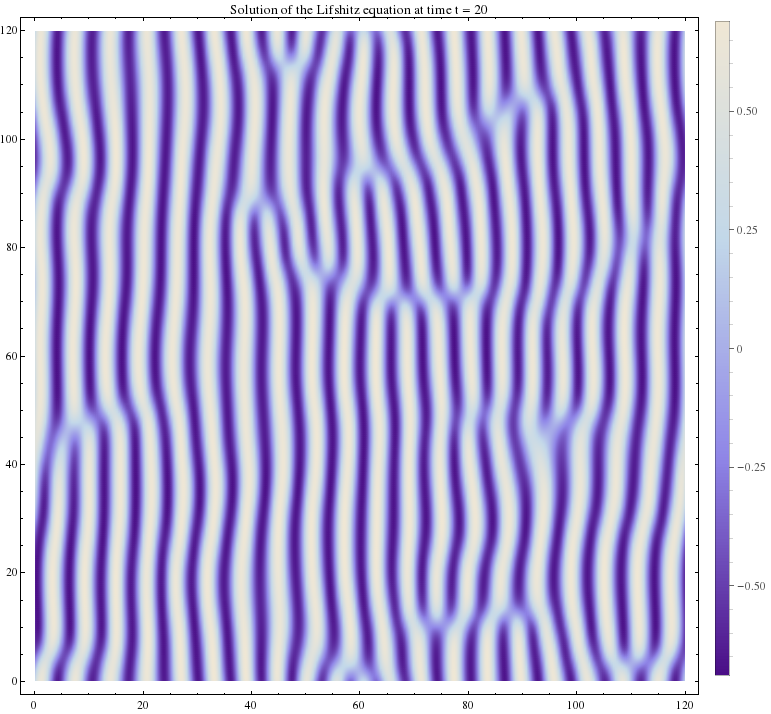
\includegraphics[width=.9\linewidth]{img/chap1/sol_Lif_t20.png}
	\caption{}
	\label{lif_t20}
	\end{subfigure}%
\begin{subfigure}{.33\textwidth}
	\centering
	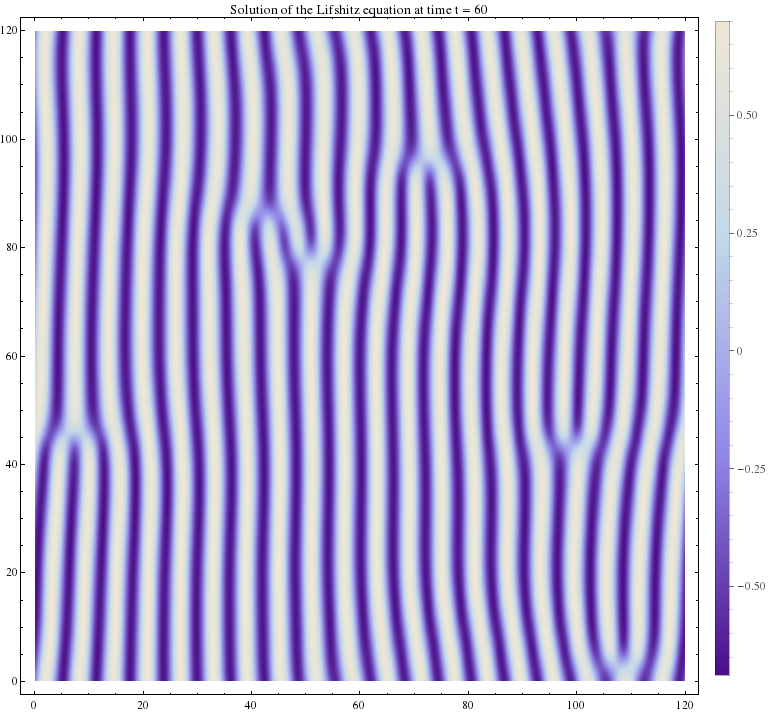
\includegraphics[width=.9\linewidth]{img/chap1/sol_Lif_t60.png}
	\caption{}
	\label{lif_t60}
\end{subfigure}%
\begin{subfigure}{.33\textwidth}
	\centering
	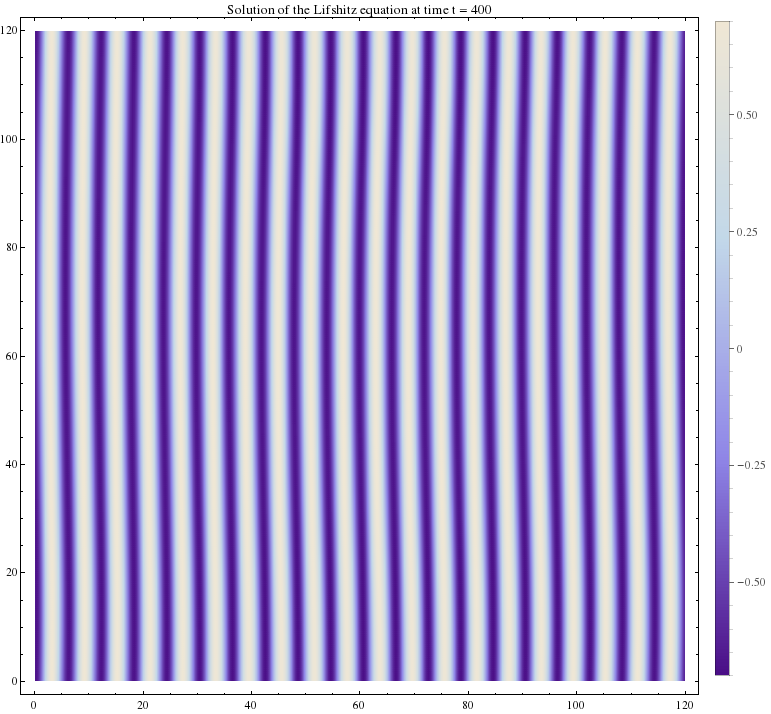
\includegraphics[width=.9\linewidth]{img/chap1/sol_Lif_t400.png}
	\caption{}
	\label{lif_t400}
\end{subfigure}
\caption{Time evolution of a field obeying the equation of movement derived from the (time dependant) Lifshitz action. We see that the field evolves toward a modulated steady state.}
\label{fig:evol_strip}
\end{figure}

The Lifshitz model aims at describing a number of physical many-body systems. They share a common intriguing feature: having a so called modulated - or stripped - phase (fig. \ref{fig:evol_strip}). In this phase, the order parameter is spatially periodic in one or several directions of space. The subspace spanned by these direction will from now be labelled $\sslash$. The hyperplan orthogonal to this modulation subspace will be labelled $\perp$.

Typically, the phase diagram of such a physical system will resemble the one presented in fig. \ref{fig:phase_diagram}.

\begin{figure}[htp]
\begin{center}
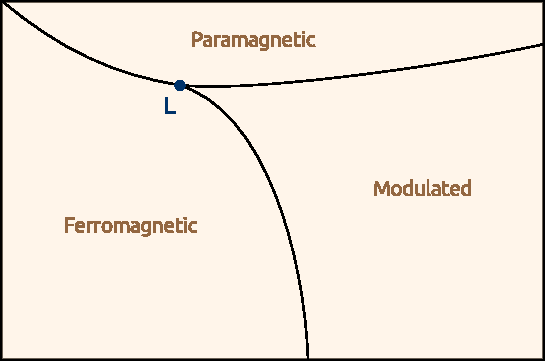
\includegraphics[scale=1]{img/chap1/phase_diagram_2.pdf}
\caption{Typical phase diagram of a system described by the Lifshitz model. The Lifshitz point is labelled $L$. ``Para'', ``Ferro'' and ``Mod'' are the abreviations for `Paramagnetic'', ``Ferromagnetic'' and ``Modulated'' respectively. Temperature varies along the vertical axis while the horizontal axis accounts for the variation of an extra parameter $\rho_0$ whose precise meaning depends on the physical nature of the studied system.}
\label{fig:phase_diagram}
\end{center}
\end{figure}

A crucial feature of this phase diagram is the critical point ($L$ in fig. \ref{fig:phase_diagram}), called the Lifshitz point. 
QUESTION : J'ai envie de dire que c'est l'un des rares exemples de point critique du second ordre qu'on trouve dans la nature, mais est-ce vrai ?
The Lifshitz point is at the intersection of two \textit{second order} phase transition lines. This is very seldomly encountered in nature. Therefore, the study of this critical point, and more precisely the determinantion of the critical exponents at this point is of particular interest.

Historically, the manganese phosphite (MnP) magnetic cristal was one of the first systems in which a Lifshitz point could be detected. Moreover, the entire phase diagram around the Lifshitz point of the MnP cristal could be inferred with high precision from experimental measurements \cite{MnP}.
In the case of the MnP magnetic cristal, the $\rho_0$ tunable parameter is an external magnetic field applied to the cristal, while the order parameter  is the local magnetization of the atoms. In the modulated phase, it is the angle between the direction of the local magnetization and a direction of reference that is spatially modulated.

Experiments also provide evidence of Lifshitz point existence in ferroelectrics and liquid cristals.

\subsubsection{The Lifshitz model}

The Lifshitz model is a field theory, describing a vector field $\phi$ whose components will be denoted $\phi_i$.
If we like to think in terms of magnetic systems, like the MnP cristal, we can say that $\phi$ is the local magnetization.
 To write the action for the Lifshitz model, we chose a basis $(\mathbf{e_n})_{1 \leq n \leq d}$. We decide that this basis is such that its first $m$ vectors span the $m$ dimensional $\sslash$ subspace, while of course the remaining $d-m$ base vector span the $\perp$ subspace. In this basis, the Lifshitz action is
\begin{equation}
S = \int_x \sum_{i=1}^N \left( \frac{1}{2} \left(\sum_{n_\perp=m+1}^{d}\frac{\partial \phi_i}{\partial x_{n_\perp}} \mathbf{e_{n_\perp}}\right)^2 + \frac{\rho_0}{2} \left(\sum_{n_\sslash=1}^{m}\frac{\partial \phi_i}{\partial x_{n_\sslash}} \mathbf{e_{n_\sslash}}\right)^2 + \frac{\sigma_0}{2} \left(\sum_{n_\sslash=1}^{m} \frac{\partial^2 \phi_i}{\partial x_{n_\sslash}^2} \mathbf{e_{n_\sslash}}\right)^2 \right) + U(\phi)
\end{equation}
As we want to model the broadest possible class of physical systems, we will say that $U$ is an almost completely arbitrary potential. We only ask for it to have the $O(N)$ symmetry, ie to be a function of
\begin{equation}
\rho \define \frac{\phi_i \phi_i}{2}
\end{equation}
From now on we will use the self-explanatory shorthand notation
\begin{equation}
S = \int_x \left( \frac{1}{2}(\p{\perp} \phi)^2 + \frac{\rho_0}{2}(\p{\sslash} \phi)^2 + \frac{\sigma_0}{2} (\p{\sslash}^2 \phi)^2 + U(\rho) \right)
\end{equation}

We see that this action closely ressemble the well known action of the $O(N)$ model
\begin{equation}
S_{O(N)} = \int_x \left( \frac{1}{2}(\partial \phi)^2 + U(\rho) \right)
\end{equation}
Namely, we recover it if we set $\rho_0 = 1$ and $\sigma_0 = 0$. We see that what differentiate the Lifshitz and $O(N)$ action is on one hand the presence a non trivial (\textit{ie} different from 1) $\rho_0$, breaking the $O(N)$ invariance, and on the other hand the presence of an extra term involving a laplacian squared. Clearly, these two modifications must be responsible for the appearance of spatially modulated structures, but why exactly? 
We can gain a useful intuition of why a spatially modulated structure is closely linked to the existence of a laplacian squared term in the action by looking at a microscopic version of our model. 

\subsection{A discrete counterpart: the anisotropic Ising model}

Stricto sensu the discrete counterpart of the Lifshitz model would be an anisotropic Heisenberg model, but to simplify things - without changing the essence of the argumentation - we consider an anisotropic Ising model instead.

First, let us consider a chain of Ising spins with the Hamiltonian
\begin{equation}
H_{\text{chain}} \define - J \sum_i S_i S_{i+1}
\end{equation}
We know that if $J$ is positive, the interaction is ferromagnetic, whereas is $J$ is negative, the interaction is antiferromegnetic. 
The antiferromagnetic order already shows some kind of spatial modulation, but it only exists at zero temperature! 
The idea to make a spatially modulated order survive at non zero temperatures is to consider a second neighbours \textit{antiferromagnetic} interaction, together with a first neighbours \textit{ferromagnetic} interaction:
\begin{equation}
H_{\text{chain}} = - J_1 \sum_i S_i S_{i+1} - J_2 \sum_i S_i S_{i+2}
\end{equation}
 The competition between ferromagnetic and antiferromagnetic interactions will produce a spatial modulation of the spins at non zero temperatures, at least for some values of the interaction strenghts ratio $J_2/J_1$. However, for a long range order to exist at finite temperature, we need to work in two dimensions or more, \textit{ie} to trade our spin chain for a spin lattice:
 \begin{equation}
 H_{\text{lattice}} \define - \sum_i \left( J_0 \sum_{\delta_\perp} S_i S_{i+\delta_\perp} + J_1 \sum_{\delta_\sslash} S_i S_{i+\delta_\sslash} + J_2 \sum_{\delta_\sslash} S_i S_{i+2 \delta_\sslash} \right)
 \end{equation}
 The existence of a stripped phase is a well known feature of this model \cite{ANNNI}, called the ANNNI (axial next-nearest neighbour Ising) model.
 
 Now, what is the link between this discrete spin lattice hamiltonian, and our continuous action?
First, note that a sum on nearest neighbours can be rewriten in terms of a discrete laplacian on the lattice, while a sum on next-nearest neighbours involves a discrete laplacian squared:
\begin{equation}
H_{\text{lattice}} = -\sum_i \left( \kappa S_i^2 + J_0 S_i \Delta_\perp S_i + (J_1 + 4 J_2) S_i \Delta_\sslash S_i - J_2 S_i \Delta_\sslash^2 S_i \right)
\end{equation}
where we introduced the differencial operators on the lattice:
\begin{align}
\Delta_\sslash S_i = \sum_{\delta_\sslash} S_{i-\delta_\sslash} - 2 S_i + S_{i+\delta_\sslash} \\
\Delta_\sslash^2 S_i = \sum_{\delta_\sslash} -S_{i-2\delta_\sslash} +  4 S_{i-\delta_\sslash} - 4 S_i + 4S_{i+\delta_\sslash} - S_{i+2\delta_\sslash}
\end{align}
This rewriting in terms of discrete differential operators makes it clear that this Hamiltonian is the discrete -microscopic- counterpart of the Lifshitz action. We now understand -at least intuitively- the origin of the spatially periodic structures (shown in fig. \ref{fig:evol_strip}) the Lifshitz field exhibit. They exist because of the competition bewtween \textit{nearest neightbours ferromagnetic interactions} (giving rise to the $\Delta_\sslash$ term in the Lifshitz action), and \textit{next-nearest neightbours antiferromagnetic interactions} (giving rise to the $\Delta_\sslash^2$ term in the Lifshitz action).

At this point a question arises: why work with a Lifshitz coarse-grained field theory, since we have a better physical understanding of an underlying microscopic model? What is more, in passing to a continuous theory, we lose informations about the microscopic underlying lattice. 
This is actually not a problem since the statistical quantities we are interested in computing -namely the critical exponents of the phase transition- are universal; they do not depend on the specific microscopic model. Actually, passing to a field theory is even advantageous as it frees us of the irrelevant microscopic details. 
Even more crucial is the fact that field theories are the objects of choice for application of the powerful methods of the renormalization group, which we will now desribe.

\chapter{Introduction to the nonperturbative renormalization techniques}

At the so-called Lifshitz critical point, three phases intersect. This is rather unsual, so we expect the physics of the vicinity of this point to be of special interest. To investigate it, we would like to compute the critical exponents associated to this transition point. To this end, we used the powerful machinery of the renormalization group, and more precisely of one particular implementation of the renormalization ideas: the nonpertubative renormalization group.

In this chapter we propose first a very general introduction to the ideas and concepts of renormalization. Then we focus on the nonperturbative renormalization group techniques.

\section{Introduction to the renormalization group}

\subsection{The renormalization procedure}

The idea of renormlization is to consider a given many-body system at different length scales. At a given length scale $S$ the system is described by an effective Hamiltonian $H_S$. 
For a many-body system, two length scales play a special role: 
\begin{itemize}
\item The microscopic length scale, $a$, which is for example for a cristal the typical distance between two neighbouring atoms.
It is convenient to define the scale in the units of the microscopic lenghtscale $a$, and this is what we are going to do. So, for example, the system at $S=3$ will mean the system at lengthscale $3 a$.
\item The macroscopic length scale $L$, which is the size of the system. 
\end{itemize}

The Hamiltonian at the microscopic length scale is simply the microscopic Hamiltonian, \textit{ie}
\begin{equation}
H_1 = H
\end{equation}
 while the Hamiltonian at the macroscopic length scale is called to effective action (and sometimes the Gibbs free energy) and is denoted $\Gamma$:
\begin{equation}
  H_{L/a} = \Gamma
\end{equation} 

For the moment what we mean by ``the Hamiltonian at a length scale $S$'' is rather vague. To be more precise, let us imagine that we want to describe a magnetic cristal. The microscopic Hamiltonian will be in general a discrete sum of local observables $O_\alpha$, depending on the value of the magnetization at site $i$, $\phi(i)$:
\begin{equation}
H[\phi] = \sum_i \sum_\alpha \kappa_\alpha O_\alpha[\phi(i), \nabla \phi(i), ...]
\end{equation}
where $\kappa_\alpha$ is the coupling constant associated to the observable $O_\alpha$. The partition function will be simply the sum over all possible configurations of the $\phi(i)$ of the Boltzmann weight associated to a given configuration:
\begin{equation}
Z = \sum_{\text{conf } \phi} e^{-H[\phi]}
\end{equation}
These equations describe the system at the microscopic scale $S=1$. Now, if we want to describe it at a scale $S \geq 1$, surely we are no longer interested in knowing the fluctuations of the field over regions of size smaller than $a S$\footnote{Experimentally, we can imagine that looking at the system at scale $S$ means probing it with devices having a spatial resolution of $a S$. Any measurement operation with such devices can be described mathematically by the convolution of an observable by an error function having a spatial support of diameter $a S$. This operation is roughtly equivalement to averaging the observables (and therefore the field) on blocks of size $a S$.}. All we need is thus the average over regions of size $a S$ of the field:
\begin{equation}
\tilde{\phi}(b) = \frac{1}{(aS)^d} \sum_{i \in B(b)} \phi(i)
\end{equation}
where $d$ is the dimension of space, and $B(b)$ is the set of sites $i$ belonging to the block $b$.

Schematically what we do is group spins by blocks of size $a S$ (fig. \ref{renorm_1}), and average over these blocks.

\begin{figure}[htp]
\centering
\begin{subfigure}{.25\textwidth}
	\centering
	
\includegraphics[width=.9\linewidth]{img/chap2/renorm_step0.pdf}
	\caption{The initial lattice.}
	\label{renorm_0}
	\end{subfigure}%
\begin{subfigure}{.25\textwidth}
	\centering
	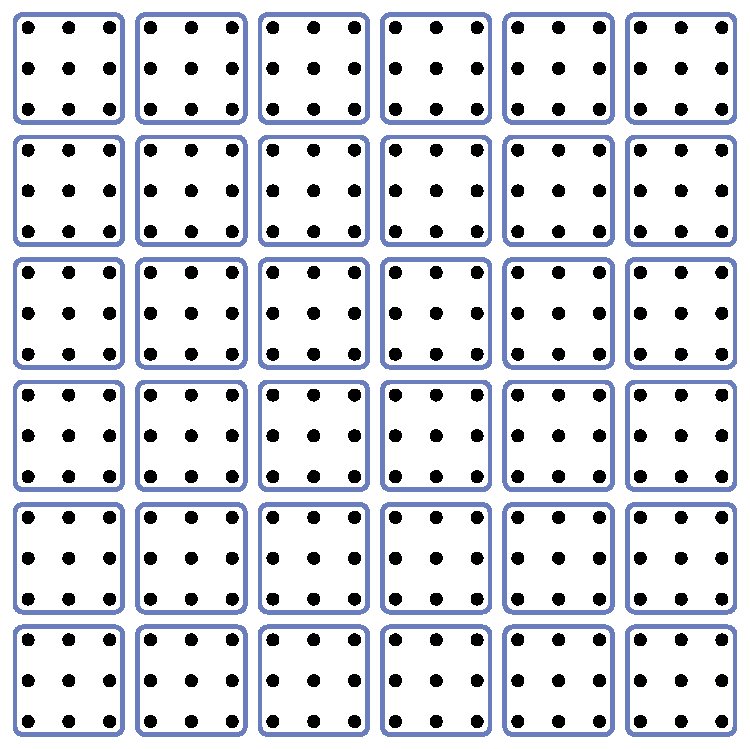
\includegraphics[width=.9\linewidth]{img/chap2/renorm_step1.pdf}
	\caption{Block spin averaging.}
	\label{renorm_1}
\end{subfigure}%
\begin{subfigure}{.25\textwidth}
	\centering
	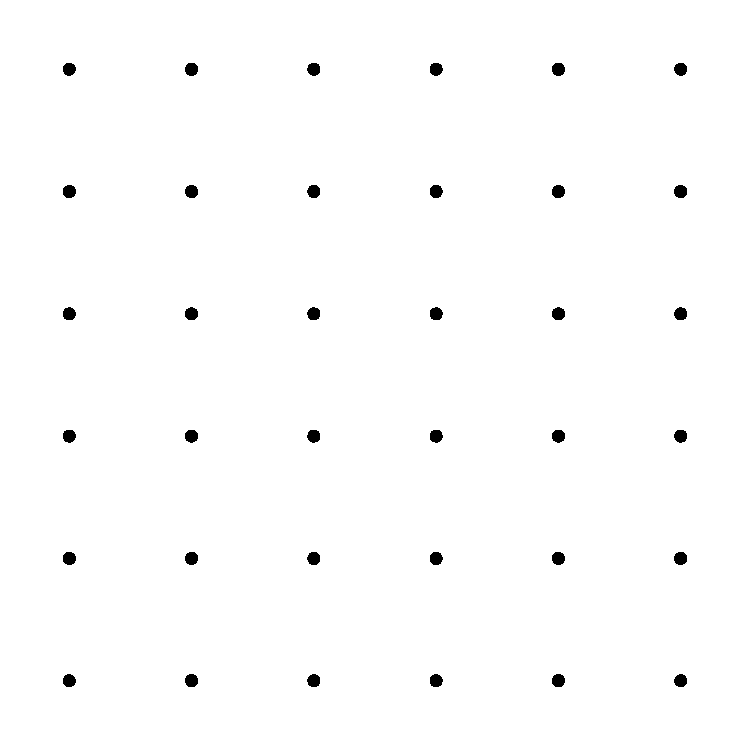
\includegraphics[width=.9\linewidth]{img/chap2/renorm_step2.pdf}
	\caption{The new lattice.}
	\label{renorm_2}
\end{subfigure}%
\begin{subfigure}{.25\textwidth}
	\centering
	
\includegraphics[width=.9\linewidth]{img/chap2/renorm_step3.pdf}
	\caption{Rescaling.}
	\label{renorm_3}
\end{subfigure}
\caption{The renormalization procedure illustrated. Here we have chosen $S = 3$.}
\label{fig:renorm_proc}
\end{figure}

Now we replace the microscopic Hamiltonian by an effective Hamiltonian for the block spin field $\tilde{\phi}$:
\begin{equation}
H[\phi] \rightarrow \tilde{H}[\tilde{\phi}] \text{ such that } e^{-\tilde{H}[\tilde{\phi}]} = \sum_{\text{conf } \phi} \prod_{b} \delta \left( \tilde{\phi}(b) - \frac{1}{S^d} \sum_{i \in B(b)} \phi(i) \right) e^{-H[\phi]}
\end{equation}
this Hamiltonian is designed such that
\begin{equation}
\sum_{\text{conf } \tilde{\phi}} e^{-\tilde{H}[\tilde{\phi}]} = Z
\end{equation}
This Hamiltonian describe the new system depicted in fig. \ref{renorm_2}. 
We are not done yet! To make the new Hamiltonian ressemble as much as possible the one we started from, we rescale all lengths (fig. \ref{renorm_3}). We also rescale the field. Formally it means that we perform the change of variables
\begin{eqnarray}
x' = x/S  \\
\phi' = S^\Delta \tilde{\phi}
\end{eqnarray}
where $x$ could be any length appearing in the Hamiltonian.

The Hamiltonian in the new variables $H'[\phi'] = \tilde{H}[\tilde{\phi}]$ is the effective Hamiltonian after the renormalization operation.  
It could seem strange that we rescaled the field as well as the lenghts. We do that in order for the new Hamiltonian to ressemble the old one as closely as possible. We are going to see on the example of the Lifshitz mean field theory how we can chose $\Delta$ for that purpose.

To conclude, the key ideas of the renormalization procedure are the averaging over block spins, and the rescaling of lengths and fields. We have described here the case of a discrete Hamiltonian, because it seemed more intuitive. But of course the ideas of renormalization are general and can as easily be applied to a continuous Hamiltonians.

\subsection{The renormalization group}

If the structure of the Hamiltonian is kept unchanged by the renormalization group procedure, \textit{ie} if
\begin{equation}
H'[\phi'] = \sum_{i'} \sum_\alpha \kappa_\alpha' O_\alpha[\phi'(i'), \nabla' \phi'(i'), ...]
\end{equation}
then the renormalization group action is a group action\footnote{Actually, invertibility cannot be guaranteed so it rather is a semigroup action, but the distinction is of no importance for us.}. The group renormalization group is completely described by its action on the coupling contants:
\begin{equation}
\kappa_\alpha \rightarrow \kappa_\alpha' \define g(\kappa_\alpha, S)
\end{equation}
The renormalization group is a multiplicative, one parameter group:
\begin{equation}
g( g(\kappa_\alpha, S_1), S_2) = g(\kappa_\alpha, S_1 S_2)
\end{equation}
These transformations are assumed to be continuous in the coupling constant. It is also very often possible to consider the scale $S$ as a continuous parameter. Then the successive application of infintesimally close renormalization group transformations generates a continuous tranjectory in the space of coupling constants. This trajectory can be parametrized by $t \define \log(S)$, an additive parameter playing the role of a time. It is often referred to as ``the renormalization group time''.

Near a phase transition or critical point, fluctuations occur at all length scales, and thus one should expect the Hamiltonian to be scale invariant. 
In terms of the renormalization group action, scale invariance simply means that
\begin{equation}
g(\kappa_\alpha, S) = \kappa_\alpha
\end{equation}
The fact that scale invariance has such a simple meaning in the renormalization group framework is an extremely good sign. It is a hint that renormalization group is a powerful tool to look for critical points.

To illustrate that, in appendix ??? (yet to be written!), we derive from very simple renormalization group arguments some useful formulas relating critical exponents.

\subsection{Renormalization procedure applied to the mean field Lifshitz theory}

As we have just seen, an operation from the renormalization group transforms our microscopic Hamiltonian $H$ into an effective Hamiltonian at scale $S$, $H_g(S)$. We hope that this operation will not change the structure of our Hamiltonian, so that we can use the tools of the renormalization group. 
Since our Hamiltonian is not isotropic (it distinguishes between the direction of the modulation $\sslash$, and the orthogonal direction $\perp$), we expect an operation of the renormalization group to change lengthscales by two different amounts in the two unequivalent directions. 
Scales in the parallel direction will be changed by a factor $S_\sslash$
 : $x_\sslash' = (S_\sslash)^{-1} x_\sslash$
, while scales on the orthogonal direction will be changed by a factor $S_\perp$ : $x_\perp' = (S_\perp)^{-1} x_\perp$.

To simplify things we can keep a single scale $S = S_\perp$, and define $\theta$ such that $S_\sslash = S^\theta$.Note that this is equivalent to changing the \textit{units} in the parallel direction: if we say that lengths in the orthogonal direction are measured in meters, then lengths in the parallel direction are measured in $(\text{meters})^\theta$.
A volume, which is normally measured in $(\text{meters})^d$ will in our new units system be measured in $(\text{meters})^{(d-m) + \theta m}$. It is as if $d$ had been replaced by
\begin{equation}
d_m = d+ m(\theta -1)
\end{equation}

We define two anomalous dimensions by
\begin{align}
\langle \phi(p_\sslash) \phi(0) \rangle_{g^*} \propto |p_\sslash|^{\eta_\sslash -4} \\
\langle \phi(p_\perp) \phi(0) \rangle_{g^*} \propto |p_\perp|^{\eta_\perp -2} 
\end{align}
where $g^*$ is a fixed point in the space of coupling constants, and the proportionality constant is independent of the scale.

But we also know that
\begin{align}
\langle \phi(p_\sslash) \phi(0) \rangle_{g^*} \propto |p_\sslash|^{\frac{2 \Delta}{\theta}} \\
\langle \phi(p_\perp) \phi(0) \rangle_{g^*} \propto |p_\perp|^{2\Delta} 
\end{align}
where $\Delta$ is the renormalization of the field : $\phi_{g(1)}(x) = S^{-\Delta} \phi_{g(S)}(Sx)$. 
Identifying these expressions for the renormalization of the correlation function with the previous ones, we can express $\Delta$ in two unequivalent ways, thus yielding a relation between $\eta_\sslash$ and $\eta_\perp$ :
\begin{equation}
\theta = \frac{2- \eta_\perp}{4- \eta_\sslash}
\end{equation}

\subsubsection{Mean field analysis}

We recall that the Lifshitz Hamiltonian is
\begin{equation}
H = \int_x \left( \frac{1}{2}(\partial_\perp \phi)^2 + \frac{\rho_0}{2} (\partial_\sslash \phi)^2 + \frac{\sigma_0}{2} (\partial_\sslash^2 \phi)^2 + U(\rho) \right)
\end{equation}

The mean field approximation consist in neglecting the fluctuations of the field. Therefore, the integration over the fluctuations performed during a renormalization group operation is trivial, and we can directly write the transformed Hamiltonian after a renormalization group operation $g(S)$ :
\begin{equation}
H'[\phi'] = \int_{x'} S^{d_m} \left( S^{-2\Delta -2} (\partial_\perp' \phi')^2 + \sigma_0 S^{-2\Delta - 4 \theta} (\partial_\sslash'^2 \phi)^2 + \rho_0 S^{-2\Delta -2 \theta} (\partial_\sslash' \phi')^2 U'(\phi') \right)
\end{equation}
This Hamiltonian must indentify with the previous one, so
\begin{equation}
\Delta = \frac{d_m -2}{2}
\end{equation}
The Lifschitz point involves a non-trivial $\sigma_0 (\partial_\sslash^2 \phi)^2$, therefore at this critical point, $\sigma_0$ must not renormalize away, which is only possible if
\begin{equation}
\theta = \frac{1}{2}
\end{equation}

In the mean field approximation, it is as if the physical dimension were
\begin{equation}
d_{\text{mean field}} = d - \frac{m}{2}
\end{equation}
We immediately deduce that the upper critical dimension\footnote{The upper critical dimension is the dimension above which mean field theory is exact, in the sense that it gives the correct critical exponents.}, which is ``normally'' 4, becomes
\begin{equation}
d_c^> = 4 + \frac{m}{2}
\end{equation}
around the Lifschitz point.

In nature, the most common case is $m=1$ (when in the modulated phase, the field is periodic in one direction of space). In that case the upper critical dimension is $d_c^> = 4.5$. When doing perturbation theory, one usually expand around the upper critical dimension, writing
\begin{equation}
d = d_c^> - \epsilon,
\end{equation} 
where $\epsilon$ is a supposedly small parameter. When $d=3$, $\epsilon = 1.5$, which is not so small. So we expect the results from perturbation theory to be rather imprecise. To better tackle this problem, it would be great to have a method that is not perturbative in the dimension. This is what the nonperturbative renormalization group method provides, as we will now see.

\section{The nonperturbative renormalization group}

\chapter{The Lifshitz model}

As we have seen, the Wetterich equation governs the flow of the scale-dependent effective action $\Gamma_t$. Solving directly this differential equation to find $\Gamma_t$, though in theory possible, is in practice very difficult. Inded the $\Gamma_t$ depends on the (background) field $\phi$, a function of the momentum. Determining completely $\Gamma_t$ requires knowing its value for all functions $\phi$. 

So, instead of solving directly the Wetterich equation, we start from a reasonable functional form for $\Gamma_t$ with unknown coefficients, we plug it in the Wetterich equation to get flow equations for this coefficients, and we solve these equations.

If we assume that it is analytic in the potential, the effective action can be written as the infinite sum
\begin{equation}
\Gamma_t[\phi] = \int_{x} \left( m_0 (\partial \phi(x))^2 + m_1 (\partial \phi(x)^2)^2 + ... + n_0 (\partial^2 \phi(x))^2 + ... + l_0 \phi(x)^2 + l_1 \phi(x)^3 +... \right)
\end{equation}

This expression can be further simplified if the system under study has some invariance properties. The simplest model having such an invariance is the Ising one, whose microscopic Hamiltonian is invariant under the action of the $\mathds{Z}_2$ symmetry group. If we chose a regulator that preserves this symmetry, it is clear that the effective action $\Gamma_t$ must also be invariant under $\mathds{Z}_2$. The most general expression for $\Gamma_t$ that preserves this symmetry is
\begin{equation}
\label{eq:ising_anzatz}
\Gamma_t^{\text{Ising}}[\phi] = \int_{x} \sum_{i,j \in \mathds{N}} Z_{t,ij} (\partial \phi(x))^{2i} \phi(x)^{2 j}
\end{equation}
The strategy is now simple:
\begin{itemize}
\item Compute $\Gamma_t^{(2)}(x,y)$ from \ref{eq:ising_anzatz}
\item Plug the result in the right hand side of the Wetterich equation
\item Deduce the flow equation for $Z_{t,ij}$: $\p{t} Z_{t,ij} = F_{i,j}\left( {Z_{t,kl}} \right)$
\end{itemize}
Following this procedure we went from a functional differential equation to a set of simple differential equations. Solving this set of flow equations give us a complete knowledge of the model. In particular solving the fixed point equations $0 = F_{i,j}\left( {Z^*_{t,kl}} \right)$ will give us access to the critical properties of the Ising model: critical exponents, critical potential,... Note that for the moment no approximations have been made!

In practice however we know that the lowest degree terms in $\partial \phi$ and $\phi$ will have the most significant contribution to the flow. Therefore we can make the approximation of cutting the development at some order. This has the great practical advantage of reducing the number of flow equations to solve to a finite number. Note that other approximation schemes are possible (development in powers of the field, BMW scheme...). We will not talk about these.

Now, let us apply this approximation scheme to the Lifshitz model.

\section{An Anzatz for the Lifshitz scale-dependant effective action}
We recall that the Lifshitz microscopic Hamiltonian is

\begin{equation}
H[\phi] = \int_x \left( \frac{1}{2}(\p{\perp} \phi)^2 + \frac{\rho_0}{2}(\p{\sslash} \phi)^2 + \frac{\sigma_0}{2} (\p{\sslash}^2 \phi)^2 + V(\rho) \right)
\end{equation}
where $\rho = \phi_i \phi_i/2$. 
The Lifshitz Hamiltonian has the $O(n)$ symmetry\footnote{Meaning that a rotation of the $n$-dimensional field $\phi$ leaves the Hamiltonian invariant: $H[\mathcal{R}(n)\phi] = H[\phi]$ if $\mathcal{R}$ is an orthogonal $n \times n$ matrix.}, therefore the scale-deendant effective action should also have this symmetry. Moreover the kinetik term in the Lifshitz Hamiltonian decomposes into two parts:
\begin{itemize}
\item $\int_{x} \frac{\rho_0}{2}(\p{\sslash} \phi)^2 + \frac{\sigma_0}{2} (\p{\sslash}^2 \phi)^2$, invariant under $\left(x_\sslash,x_\perp \right) \rightarrow \left(\mathcal{R}(m) x_\sslash, x_\perp\right)$
\item $\int_{x} \frac{1}{2}(\p{\perp} \phi)^2$, invariant under $\left(x_\sslash,x_\perp \right) \rightarrow \left(x_\sslash, \mathcal{R}(d-m) x_\perp\right)$
\end{itemize}
Since the scale-dependant effective action must satisfy these symmetry properties, its most general form is
\begin{equation}
\Gamma_k[\phi] = \int_{x} U(\rho) + \left( \frac{1}{2} Z_\perp(\rho) (\partial_\perp \phi)^2 + \frac{1}{4} Y_\perp(\rho) (\partial_\perp \rho)^2 + ... \right) + \left( \frac{1}{2} \rho_0(\rho) (\partial_\sslash \phi)^2 + ... \right) + \left( \frac{1}{2} Z_\sslash(\rho) (\partial_\sslash^2 \phi)^2 + ... \right)
\end{equation}

It turns out to be a very good approximation to cut the derivative expansion to first order \footnote{To compute critical exponents, one does not need to take into account the full momentum dependence of the theory. However for computing correlation function the momentum dependence is essential. Were we to compute these quantities, we will probably have to go further in the derivative expansion}. That is to say, we make the approximation
\begin{eqnarray}
\frac{1}{2} Z_\perp(\rho) (\partial_\perp \phi)^2 + \frac{1}{4} Y_\perp(\rho) (\partial_\perp \rho)^2 + ...  \simeq  \frac{1}{2} Z_\perp(\rho) (\partial_\perp \phi)^2  \\
 \frac{1}{2} \rho_0(\rho) (\partial_\sslash \phi)^2 + ...  \simeq  \frac{1}{2} \rho_0(\rho) (\partial_\sslash \phi)^2 \\
\frac{1}{2} Z_\sslash(\rho) \partial_\sslash^2 \phi)^2 + ... \simeq \frac{1}{2} Z_\sslash(\rho) \partial_\sslash^2 \phi)^2
\end{eqnarray}
Moreover, we make the approximation that the field renormalizations $Z_\perp(\rho)$, $\rho_0(\rho)$ and $Z_\sslash(\rho)$ do not depend on the field. So, the definitive form of the Anzatz we chose for $\Gamma_t$ is
\begin{equation}
\label{eq:gamlif}
\Gamma_t[\phi_i] = \int_x \left ( \frac{Z_\perp}{2} (\partial_\perp \phi)^2 + \frac{\rho_0}{2} (\partial_\sslash \phi)^2 + \frac{Z_\sslash}{2} (\partial_\sslash^2 \phi)^2 + U(\rho) \right )
\end{equation}
This is the form of the Lifshitz scale-dependent effective action we have worked on during this internship.
Though this does not appear explicitly, the field renormalizations and the effective potential $U$ depend on the renormalization time $t$. As we are going to see, the $t$ dependence of $Z_\perp$ and $Z_\sslash$ gives rise to non trivial anomalous dimensions. The anomalous dimensions are expected to act as a small correction to the value of the critical exponents. At first order, we can thus assume trivial anomalous dimensions. This amounts to forgetting the $t$ dependence of $Z_\sslash$ and $Z_\perp$ in the effective action. This approximation is called the \textit{local potential approximation}.


 We will now make use of the Wetterich equation to know how this quantities change through the renormalization process. Then we will use this knowledge to derive the critical exponents.

\section{The Lifshitz renormalization flows}

\subsection{Dimension-driven versus fluctuations-driven flows}
We recall that looking at the mean field version of a theory consists in neglecting all fluctuations of the field. Therefore, in the case of a mean field theory, the renormalization procedure - average on fluctuations up to a certain scale, definition of an effective Hamiltonian and rescaling - only requires rescaling. 
The conclusion is that the renormalization flows of mean field theories' coupling constants are only due to their dimension.

If we wish to go beyond the mean field approximation, we have to take into account the fluctuations of the field.
They are often small compared to the mean value of the field, meaning that their contribution to the flows will be small compared to the contribution coming from the mean field theory. In other words, the fluctuation-driven part of a renormalization flow is generally small compared to its dimension-driven part. 
Wishing to concentrate on the small non-trivial part of the flow: the fluctuation-driven part, we define \textit{dimensionless coupling constants}, that are by construction subject to a fluctuation-driven flow only.\footnote{Numerically, if we want to track the contribution to the flow of fluctuations $10^{12}$ weaker than the mean field contribution, we must achieve at least $12$ digits precision, which is often rendered impossible by rounding errors. In this context using dimensionless coupling constant indeed seems an excellent idea!}

With these ideas in mind, we define the following dimensionless quantities 


\begin{center}
\begin{tabular}{|c|c|c|}
\hline
$q_\sslash^2 = k^{2 \theta} y_\sslash$ & $q_\perp^2 = Z_\sslash Z_\perp^{-1} k^{4\theta} y_\perp$ & $\rho_0 = Z_\sslash k^{2\theta} \bar \rho_0$\\ 
\hline 
$R(q_\perp^2,q_\sslash^2) = Z_\sslash k^{4\theta} y_\sslash^2 r(y_\perp, y_\sslash)$ & $U(\rho) = Z_\sslash k^{d_m} u(\bar{\rho})$ & $\rho = Z_\sslash^{-1} k^{-4\theta + d_m} \bar{\rho}$ \\ 
\hline 
\end{tabular}
\end{center}

Note that given the relation
\begin{equation}
\theta = \frac{2-\eta_\perp}{4-\eta_\sslash}
\end{equation}
we have a certain liberty relative to the adimensionning of the physical quantities. For example we can define $\rho_0 = Z_\sslash k^{2\theta} \bar{\rho_0}$ or $\rho_0 = Z_\perp^{1/2}Z_\sslash^{1/2}k\bar{\rho_0}$. These two definitions lead to two different $\bar{\rho_0}$ functions, but the two functions have \textit{the same dimensional flow}.. Here we chose the adimensionning such that $Z_\sslash$ simplifies everywhere in the propagators. 

\subsection{Flow of the potential}
From the shape of the potential, we can tell in which phase we are. Therefore knowing how the potential changes with $t$ is of paramount importance. We shall thus start with the derivation of the flow equation for the potential.

We see that 
\begin{equation}
U(\rho_0) = \delta(0)^{-1} \Gamma_t[ \phi] |_{\phi(x) = \phi_0}
\end{equation}
where $\phi_0$ is some uniform (in direct space) configuration of the field, and where $\rho_0 = \phi_{0i} \phi_{0i}/2$. Note that if we were to work on a finite-size system, the $\delta(0)^{-1}$ term would be replaced by the volume of the system. Therefore it plays the role of the system volume for the infinite size system we consider here.

We take a derivative with respect to $t$ to get an expression for the flow of the potential, and we plug in the Wetterich equation on the right hand side:
\begin{equation}
 \partial_t U(\rho_0) = \delta(0)^{-1} \partial_t \Gamma = \frac{1}{2 \delta(0)} \hat \partial_t \tr{\log\left( \Gamma_t^{(2)} + R_t  \right)}
\end{equation}
This is the flow equation for the potential!\footnote{It should be noted that we only derived the flow equation of the potential for a constant field configuration. This is of no importance as we do not need the \textit{functional} dependence of the potential, $(x \mapsto \rho(x)) \mapsto U(\rho(x))$ but only its ``digital'' dependence $\rho_0 \mapsto U(\rho_0)$ to characterize it completely.}

From eq. \ref{eq:gamlif} we compute the first functional derivative of the Lifshitz effective action:
\begin{equation}
\frac{\delta \Gamma_t}{\delta \phi_i(x)}[\phi] = - Z_\perp \Delta_\perp \phi_i(x) - \rho_0 \Delta_\perp \phi_i(x) + Z_\sslash \Delta_\sslash^2 \phi_i(x) + U'(\rho) \phi_i(x)
\end{equation}
taking a second functional derivative with respect to the field:
\begin{equation}
\frac{\delta^2 \Gamma_t}{\delta \phi_i(x) \delta \phi_j(y)}[\phi] =\left(   \delta_{ij} \left( - Z_\perp \Delta_\perp - \rho_0 \Delta_\perp + Z_\sslash \Delta_\sslash^2  + U'(\rho) \right) + U''(\rho) \phi_i(x) \phi_j(y) \right) \delta(x-y)
\end{equation}
and passing to Fourier space:
\begin{equation}
\frac{\delta^2 \Gamma_t}{\delta \phi_i(p) \delta \phi_j(q)}[\phi] \define \Gamma^{(2)}_{ij}(p,q) = 
\left( \delta_{ij} \left(Z_\perp p_{\perp}^2 +\rho_0 p_{\sslash}^2 +Z_\sslash (p_\sslash^2)^2 + U'(\rho (x))\right)+\phi_i(p) \phi_j(q) U''(\rho (x)) \right) \delta(p+q)
\end{equation}
We can decompose the two-points 1-particle irreducible function $\Gamma^{(2)}_{ij}$ on a orthogonal projectors along the direction of the field and orthogonal to it:
\begin{align}
\Pi^a_{i,j} = \delta_{ij} - \frac{\phi_i \phi_j}{2 \rho} \\
\Pi^r_{i,j} = \frac{\phi_i \phi_j}{2 \rho}
\end{align}
thus allowing us to easily write the regularized propagator appearing in the Wetterich equation:
\begin{equation}
\left( \Gamma^{(2)}_{ij}(p,q) + R_t(p,q) \right)^{-1} = \left( G_a(q) \Pi^a_{ij} + G_r(q) \Pi^r_{ij} \right) \delta(p+q)
\end{equation}
where we used the radial and angular propagators:
\begin{align}
G_r(q)_{i,j} \define \frac{1}{Z_\sslash q_\sslash^4 + Z_\perp q_\perp^2 + \rho_0 q_\sslash^2 + R_t(q)  + U'(x) + 2 \rho U^{(2)}(\rho)} \\
G_a(q)_{i,j} \define \frac{1}{Z_\sslash q_\sslash^4 + Z_\perp q_\perp^2 + \rho_0 q_\sslash^2 + R_t(q) + U'(\rho)}
\end{align}
and chosen the regulator to be diagonal:  $R_{t,ij}(q) = R_t(q) \delta_{ij}$.
We can now rewrite in a more explicit way the Wetterich equation:
\begin{equation}
\p{t} \Gamma_t = \frac{1}{2} \int_q \left(  G_a(q) \Pi^a_{ij} + G_r(p) \Pi^r_{ij} \right) \p{t} R_{t,ij}(q)  = \frac{1}{2} \int_q \left(  G_a(q) + (n-1)G_r(p) \right) \p{t} R_{t}(q) 
\end{equation}
Note that the radial (massive) propagator appears once whereas the angular (massless) propagator appears $n-1$ times in the flow equation. This is of course because as soon as we choose a direction for the field $\phi$, the  $O(n)$ invariance is no longer explicit (though the equation is of course still $O(n)$ invariant). Therefore, a massive Goldstone mode and $n-1$ massless modes appear, in accordance with Goldstone's theorem.

Imposing now that the field is constant, we have for the flow of the potential
\begin{equation}
\p{t} U(\phi_0) = \frac{1}{2} \int_q \left( G_r(q)\atpt{unif} + (n-1)G_a(q)\atpt{unif} \right) \p{t} R_t(q)
\end{equation}
This is as far as we can get without giving explicitly a form to the regulator. 
At this point, it is a customary procedure to introduce standard functions called \textit{threshold functions} in order to lighten the notations.

The flow of the potential can be expressed in terms of the $l$ threshold function:\footnote{Definitions of the threshold functions used here can be found in appendix \ref{app:thresholds}.}
\begin{equation}
\p{t}U = 8 v_m v_{d-m} k^{d_m} \left( l_0^{dm}\left(u'(\bar{\rho}) + 2 \bar{\rho} u''(\bar{\rho}) \right) + (N-1)l_0^{dm}\left(u'(\bar{\rho})\right) \right)
\end{equation}
Note that the argument of the two threshold functions is dimensionless.

The flow of the dimensionless potential reads
\begin{equation}
d_t u(\bar{\rho}) = -d_m u(\bar{\rho}) +(\theta \eta_\sslash + d_m - 4 \theta) \bar{\rho} u'(\bar{\rho}) + \p{t} u(\bar{\rho})
\end{equation}
Dropping the bars everywhere, we have for the dimensionless potential,
\begin{equation}
\label{eq:flow_u}
d_t u(\rho) = -d_m u(\rho) +(\theta \eta_\sslash + d_m - 4 \theta) \rho u'(\rho) + 8 v_m v_{d-m} \left( l_0^{dm}\left(u'(\rho) + 2 \rho u''(\rho) \right) + (n-1)l_0^{dm}\left(u'(\rho)\right) \right)
\end{equation}

The fixed point potential therefore verifies
\begin{equation}
0 = u(\rho) - a(d_m, \theta, \eta_\sslash) \rho u'(\rho) - b(d, m) 
\left( l_0^{dm}\left( u'(\rho) + 2 \rho u''(\rho) \right) + (n-1)l_0^{dm}\left( u'(\rho) \right) \right) 
\end{equation}
where 
\begin{align}
a = \frac{\theta \eta_\sslash + d_m - 4 \theta}{d_m} \\
b = \frac{8 v_m v_{d-m}}{d_m}
\end{align}

Numerically, the the fixed point potential equation is not nice because it is an implicit differential equation
$0 = F(\rho ; u, u', u'')$.
However we can put it the form
$u(\rho) = f(\rho; u', u'')$.
This indicates that, by differentiation with respect to $\rho$, we can produce an \textit{explicit} equation on $v(\rho) \define u'(\rho)$:
\begin{equation}
0 = (1-a) v - a \rho v' + b \left( l_1\left(v+2\rho v'\right)\left(3v'+2\rho v''\right) + (N-1)l_1\left(v\right)v' \right)
\end{equation}
a second order, explicit differential equation on the derivative of the potential.

\subsection{Flow of the field renormalization.}

The field renormalizations are the prefactors $\rho_0$, $Z_\sslash$ and $Z_\perp$. We will see that the flows of $Z_\sslash$ and $Z_\perp$  are related to the anomalous dimensions in the parallel and perpendicular directions respectively. Therefore computing their flows is essential. 

\subsection{The anomalous dimension in the orthogonal direction.}

We note that
\begin{equation}
\label{eq:etaperp}
\frac{d}{dp_\perp^2} \Gamma^{(2)}_{ij}(p,q) = \delta_{ij} \delta(p+q) Z_\perp
\end{equation}
From that we can compute the flow of $Z_\perp$. Note that this flow depends on the impulsion $p$. From dimensional analysis it is easy to see that
\begin{equation}
 Z_\perp \xrightarrow[p \rightarrow 0,\text{~} k>0]{} C k^{-\eta_\perp}
 \end{equation} 
 where $C$ is a dimensionless constant factor. So, at vanishing $p$, the flow of $Z_\perp$ is linked to the anomalous dimension:
 \begin{equation}
 - \p{t} \log Z_\perp \xrightarrow[p \rightarrow 0,\text{~} k>0]{} \eta_\perp
 \end{equation}
 We shall use this relation to compute the anomalous dimension from the flow of $Z_\perp$.
 To express $\eta_perp$ we can simply take the limit of vanishing external moment of equation $\ref{eq:etaperp}$. This gives
\begin{equation}
\eta_\perp = -\frac{1}{\delta(0) Z_\perp} \p{t} \lim_{p \rightarrow 0} \frac{d}{dp_\perp^2} \left( \Gamma^{(2)}_{ii}(p,-p) \atpt{unif} \right)
\end{equation}
The index $i$ is still not fixed. To set things, we decide that $1$ is the direction of the uniform field $\phi_0$. Then we can either chose $i=1$, or $i \neq 1$ (all directions orthogonal to the field are equivalent). We made here the choice $i \neq 1$, because we know that in that case the expression we obtain for $\eta_\perp$ is exact in the $n \rightarrow \infty$ limit. Explicitly, we chose $i=2$.
Now all we need to do to obtain the explicit expression of $\eta_\perp$ in terms of the propagators is compute $\p{t} \Gamma^{(2)}_{22}(p,-p) \atpt{unif}$, derive it with respect to $p_\perp$ and take the limit of vanishing $p$. As the computation is rather lengthy, we will only give the important intermediate steps.

\subsubsection{Computation of $\p{t} \Gamma^{(2)}_{22}(p,-p) \atpt{unif}$}
Notice that we can intertwine $\p{t}$ and $\atpt{unif}$ since the uniform field does not flow. We will thus compute
\begin{equation}
\p{t} \left ( \Gamma^{(2)}_{22}(q,-q) \atpt{unif} \right ) = \left ( \p{t} \Gamma^{(2)}_{22}(q,-q)  \right )\atpt{unif}  = \left( \frac{\delta^2}{\delta \phi_2(p) \delta \phi_2(-p)} \p{t} \Gamma \right) \atpt{unif}
\end{equation}
Only two terms contribute to $\frac{\delta^2}{\delta \phi_2(p) \delta \phi_2(-p)} \p{t} \Gamma$. They can be written as diagrams

TODO: draw the diagrams

Note that the dependence on the external impulsion $p$ in the second diagram is entirely contained in the vertex $\Gamma^{(4)}$. Since here (because of our choice of kinetic terms in the effective action), every $n$-points function for $n \geq 3$ is momentum independent, this second diagram does not contribute to the anomalous dimensions.
So we keep only the first diagram, whose contribution to $\p{t} \left ( \Gamma^{(2)}_{2,2}(q,-q) \atpt{unif} \right )$  we call $D(p)$. We have
\begin{equation}
D(p) = \frac{-1}{2} \hat{\p{t}} \tr{ G(\cdot)\Gamma^{(3)}_{\cdot 2 \cdot}(\cdot, \cdot + p) G(\cdot + p) \Gamma^{(3)}_{\cdot 2 \cdot}(\cdot + p, \cdot) }
\end{equation}
where $G_{i,j}(p,q) = \left ( \Gamma^{(2)}_{i,j}(p,q) + R(p)\delta(p+q)\delta_{i,j} \right )^{-1}$ is the full propagator.

Now we perform the sum on discrete indices. Explicitely,
\begin{equation}
G(\cdot)_{i,j} \Gamma^{(3)}_{j,k,2} G(\cdot + p)_{k,l} \Gamma^{(3)}_{l,i,2}  = \left(G_r(\cdot) \Pi^r_{i,j}+ G_a(\cdot) \Pi^a_{i,j} \right) \Gamma^{(3)}_{j,k,2} \left(G_r(\cdot+p) \Pi^r_{k,l}+ G_a(\cdot+p)\Pi^a_{k,l}\right) \Gamma^{(3)}_{l,i,2} 
\end{equation}
We have
\begin{equation}
\Gamma^{(3)}_{i,j,2} = \sqrt{2 \rho} U^{(2)}(\rho) \left( \delta_{i,1}\delta_{k,2} + \delta_{i,2}\delta_{k,1} \right)
\end{equation}
The computation is not as tedious as it may seem, because the action of the projectors on $\Gamma^{(3)}_{ij2}$, itself a projector, is simple. We realize that only cross terms in the previous expression are non zero.
So, finally,
\begin{align}
\eta_\perp = \frac{1}{Z_\perp} \tr{\Pi^r \Gamma^{(3)} \Pi^a \Gamma^{(3)}} \hat{\p{t}} \lim_{p \rightarrow 0} \frac{d}{dp^2_\perp} \int_q G_r(q) G_a(p+q)
\end{align}
This is a very general expression, completely independent of the form of the effective action, as long as it has no kinetic terms of order $\geq 3$ in the field. In particular, it expressions also holds for the $O(n)$ model.

More specifically here we have
\begin{equation}
\tr{\Pi^r \Gamma^{(3)} \Pi^a \Gamma^{(3)}} = 2 \rho \left ( U^{(2)}(\rho) \right )^2
\end{equation}

\subsubsection{Action of the derivative with respect to the momentum}
Computing the derivative is a lengthy, error-prone computation. I used Mathemtica to do it. The procedure is explained in appendix ??? to be written.
Identifying with the threshold functions, we have finally
\begin{equation}
\eta_\perp = 16 v_m v_{d-m} \frac{2 \rho \left( U^{(2)}(\rho) \right)^2}{(d-m)Z_\perp} \left( 2 K_{0,2120} - 4 M_{0,3120} + (d-m)N_{0,2100} \right)
\end{equation}

Actually the $K$ function can be re-expressed in terms of $M$ and $N$ functions by integration by part:
\begin{equation}
K_{0,mn\alpha \beta} = -\left(\frac{d-m+\alpha}{2}-1\right) N_{0,mn \alpha-2 \beta} + m M_{0,m+1 n \alpha \beta} + n M_{0,m n+1 \alpha \beta}
\end{equation}
Applying this formula permits us to express the orthogonal anomalous dimension in a rather compact form
\begin{equation}
\label{eq:flow_perp}
\eta_\perp = 64 v_m v_{d-m} \frac{ \rho \left( U^{(2)}(\rho) \right)^2}{(d-m)Z_\perp} M_{0,2220}
\end{equation}

\subsection{The anomalous dimension in the parallel direction, and the flow of $\rho_0$.}

The two other computations are very similar. In particular the flow of $\rho_0$ should be given by the flow of $Z_\perp$ with the role of the $\perp$ and $\sslash$ directions exchanged, because of the symmetry between $\rho_0$ and $Z_\perp$. The formula for $\eta_\sslash$ is more complicated as it involves fourth powers of the momentum.
\begin{align}
\label{eq:flow_rho_ss}
d_t \rho_0 = -\theta \left(2-\eta_\sslash\right) \rho_0 - \frac{16 v_{d-m} v_m}{m} 2 \rho \left( u^{(2)}(\rho) \right)^2 2 M_{1,2202} \\
\eta_\sslash = 16 v_{d-m} v_m 2 \rho \left( u^{(2)}(\rho) \right)^2 
\Bigg[ M_{1,3100} - \frac{1}{2} K_{1,2100} + \frac{1}{m}\left( -12 S_{1,4102} + 12V_{1,31002} -2W_{1,2102} \right) \\
{}+ \frac{1}{m(m+1)}\left( 48 T_{1,5104} -72 Z_{1,4104} +12 U_{1,3104} +16 Y_{1,3104} -2 X_{1,2104} \right) \Bigg]
\end{align}

Equations \ref{eq:flow_u}, \ref{eq:flow_perp}, \ref{eq:flow_rho_ss} tell us how the potential, $\rho_0$ and the anomalous dimensions are modified under the action of the renormalization group. We now are interested in computing the critical exponents of the Lifshitz critical point (the meeting point of the paramagnetic, ferromagnetic and modulated phases). 

\Chapter{Conclusion}{}

During this internship, I discovered a domain of physics I new nothing about before. 
We are only beginning to understand the strange physics of granular materials, and it was exciting to be part of this adventure for a few weeks. I feel like I only scratched the surface of the subject, and yet I learned an enormous amount of physics, mathematical techniques and programming during my internship. 
I learned about how to describe and model granular flows. I learned about the mathematical difficulties arising from these models\footnote{namely ill-posedness. I chose not to talk about it in this report, as it is not required to understand the segregation equation, which is the central equation studied during my internship.}. I also learned about the strange phenomenon of segregation, and how to model it. It is then that I read about the mathematical theory of hyperbolic partial differential equations, and how to solve this type of equations numerically.

The main goal of my internship was to develop a code to solve the 3D segregation equation. 
At the end, the code could be used to solve systems of hyperbolic equations
\begin{equation}
	\begin{matrix}
	\p{}{t} u_1 + \sum_{i=1}^n \p{}{x_i} f_{1i}(\mathbf{u}, \mathbf{x}) = 0 \\
	\vdots \\
	\p{}{t} u_m + \sum_{i=1}^n \p{}{x_i} f_{mi}(\mathbf{u}, \mathbf{x}) = 0 \\
\end{matrix}
\end{equation}
where $\mathbf u(t, \mathbf x)$ is the unknown $m$-dimensional field living in a $n$-dimensional space (in our case, it is the scalar field $\phi$ living in a 3D space). Since it is very general, one can use this code to solve a lot of different physical problems, and it will be re-used later on.

During the last two weeks of my internship, I took interest in the theoretical side of the problem: namely, how to explain analytically the spiralling structure observed in the simulations and the experiments. Although I did not succeed in doing it, it was really interesting to learn how to solve hyperbolic equations. In particular, I was fascinated by the elegance of the change of coordinates used to solve 2D segregation equations, as detailed in appendix \ref{app:char}. 

It was my job as an intern to do simulations and analytical computations. But I also had the great opportunity to toy with some of the small-scale granular experiments hosted in the University of Manchester. 
This internship made me understand the fundamental importance of the interplay between experiments, simulations and analytical computations. 

 
\appendix
\documentclass[11pt]{book}
\usepackage[left=2cm,right=2cm,top=2cm,bottom=2cm]{geometry}
%Gummi|061|=)
\title{\textbf{Segregation theory}}
\author{Nicolas}
\date{}
\usepackage{amsmath}
\newcommand{\om}[1]{\ensuremath{ \mathcal{O} \left( {#1} \right) }}
\begin{document}

\chapter{Segregation theory}

\section{Physical context}

In this appendix, I will give a simple derivation of the equation we used to model the segregation process taking place in granular flows.

We consider a granular flow going down a slope (FIG). For the sake of simplicity, I will assume that the granular material is a mixture of small and large particles. This assumption is commonly made, since it simplifies greatly the equations, but still captures the essential physical features of segregation. For a more general theory, see CIT.
As usual, we model the granular flow using the tools of continuum mechanics. 

The idea is to see the set of large particles in the material as a matrix through the holes of which small particles can fall. 
If the material is a still, initially homogeneous mixture of small and large particles, it will partially segregate (FIG: leaving the uppermost layers full of large particles, the lowermost full of small particles.). In this case middle layers are a mixture of small and large particles.
If the material is a flowing, initially homogeneous mixture of small and large particles, it will completely segregate (FIG). This is because as the material flows down the slope, the local void ratio of the large particles matrix fluctuate, causing small to fall into newly opening gaps. The result is a progressive migration of small particles to the bottom. Because of force imbalance, large particles are pushed upward as small particles go downward. In the end, the material is constituted of a layer of pure large particles topping a layer of pure small particles.

\section{Derivation of the segregation equation}

Let us start by writing down the momentum and force balances for each one of the 2 constituents

\begin{equation} \label{eq:mom_bal}
	\partial_t \rho^\nu u_i^\nu + \partial_j \rho^\nu u_i^\nu u_j^\nu = -\partial_i p^\nu + \rho^\nu g_i + \beta^\nu_i 
\end{equation}
where
\begin{itemize}
\item $\rho^\nu$ is the density of the constituent $\nu$, ie the mass of constituent $\nu$ per unit volume:

\[
\rho^\nu = n^\nu m^\nu
\]
where $m^\nu$ is the mass of a particle of the constituent $\nu$ and $n^\nu$ the number of particles of the constituent $\nu$ per unit volume
Note that if $d\tau$ is a small volume, $d\tau^\nu$ the fraction of this small volume occupied by the constituent $\nu$, and $\rho^{*\nu}$ the intrinsic density of constituent $\nu$, 

\begin{equation} \label{eq:1}
\rho^\nu = \frac{d\tau^\nu}{d\tau} \rho^{*\nu} = \phi^{\nu} \rho^{*\nu}
\end{equation}
$\phi^\nu$ is called the \textit{volume fraction} of constituent $\nu$. This expression for $\rho^\nu$ will be useful later.

\[
\rho^s + \rho^l = \frac{d\tau^s + d\tau^l}{d\tau} = \rho
\]

\item $u^\nu$ is the velocity of constituent $\nu$ averaged on the volume $d\tau$

\item $p^\nu$ is the partial pressure of the constituent $\nu$. For convenience we will define $f^\nu$ as
\begin{equation}
p^\nu = f^\nu p
\end{equation}

\item $\beta^\nu$ is the force exerted by the other constituent on the constituent $\nu$.
\end{itemize}

We assume that each constituent has the same intrinsic density: $\rho^{*s}=\rho^{*l}=\rho$. This is usually a good approximation for granular materials. In our case, DAT.

We can consider the set of large particles as a matrix inside the holes of which small particles are percolating (flowing downwards).
It is as if small particles were flowing through a porous medium. In that case, we know that the force exerted by the medium on the particles is 
\begin{equation}
\beta^s = p \partial_i f^s - \rho^s c (u^s_i - u_i)
\end{equation}
this form for $\beta$ is known as Darcy's law, and is frequently used, for example to model the percolation of water through sand.

Symmetrically, we can consider the set of small particles as a matric inside which large particles are percolation (upwards, this time), and we have
\begin{equation}
\beta^l = p \partial_i f^l - \rho^l c (u^l_i - u_i)
\end{equation}

Segregation is a gravity-induced effect. It will happen in the vertical direction. This means that if $w$ is the velocity component along vertical axis,
\begin{align} \label{eq:vel_asump}
u^\nu = u \\
v^\nu = v \\
w^\nu \neq w
\end{align}
It also follows from this asumption that 
\begin{align} \label{eq:forces_asump}
\beta^\nu_x = 0 \\
\beta^\nu_y = 0 \\
\beta^\nu_z \neq 0
\end{align}
In our case $w$ is not quite along vertical axis, because of the small angle $\theta$ the base of the inclined plan makes with the horizontal direction. 
However, \cite{eq:vel_asump} and \cite{eq:forces_sump} are still valid at first order in $\theta$, so we will assume they still hold.

Thus, we will know focus on the projection along $Oz$ of \cite{eq:mom_bal}:
\begin{equation} \label{eq:z_proj}
	\partial_t \rho^\nu w^\nu + \partial_j \rho^\nu w^\nu u_j^\nu = -\partial_z \left( p f^\nu \right) - \rho^\nu g \cos \theta + \beta^\nu_z 
\end{equation}
which, making use of Darcy's law for $\beta$ we can rewrite as
\begin{equation} 
	\partial_t \rho^\nu w^\nu + \partial_j \rho^\nu w^\nu u_j^\nu = -f^\nu \partial_z p  - \rho^\nu g \cos \theta - \rho c (w^\nu - w)
\end{equation}

In shallow waters, vertical pressure gradient $ \partial_z p $ is approximately hydrostatic. This follows from the fact that acceleration in the $Oz$ direction is very small compared to vertical pressure gradient. 
This assumption allows us to simplify our previous equation:
\begin{equation} \label{eq:z_proj}
	0 = -f^\nu \rho g \cos \theta - \rho^\nu g \cos \theta - \rho c (w^\nu - w)
\end{equation}
Now let us see why, in shallow waters, this assumption is true. If you do not want to read the proof, you can jump directly to the next subsection.

\subsection{Shallow flows}
For the sake of simplicity we will assume that acceleration in $Oy$ direction is zero: $ \partial_y v = 0 $.

Let $\Delta x$ and $\Delta z$ be the typical vertical and horizontal extent of the flow. Assuming that the flow is shallow is equivalent to saying that 
\begin{equation}
	\Delta z \ll \Delta x
\end{equation} 
This and incompressibility, are the two key assumptions we will need to prove our statement. 
Let $U$ and $W$ be the typical value of $u$ and $w$. We have
\begin{align}
	\frac{U}{\Delta x} = \om{ \frac{\partial u}{\partial x} } \\
	\frac{W}{\Delta z} = \om{ \frac{\partial w}{\partial z} }
\end{align}
Using incompressibility, we have
\begin{equation}
	\frac{\partial u}{\partial x} = \om{ \frac{\partial w}{\partial z} } 
\end{equation}
ie
\begin{equation} \label{eq:incomp}
	\frac{U}{\Delta x} = \frac{W}{\Delta z}
\end{equation}
Using momentum and forces balances \textit{for the mixture of the two components}, in projection along $Ox$ gives
\begin{equation}
	\rho \left( u \partial_x u + w \partial_z u \right) = -\partial_x p +g \sin \theta
\end{equation} 
$g \sin \theta$ is very small compared to pressure gradient, since $\theta$ is close to $0$. Thus we have
\begin{equation}
	\om{ \rho \left( u \partial_x u + w \partial_z u \right) } =  \om{ -\partial_x p }
\end{equation}
ie
\begin{equation} \label{eq:om_pressure}
	 \frac{\rho U^2}{\Delta x} = \frac{p}{\Delta x}
\end{equation}
Now using momentum and forces balance for the mixture, in projection along $Oz$ we have
\begin{equation} \label{eq:z_momentum}
	\rho \left( u \partial_x w + w \partial_z w \right) = -\partial_z p -g \cos \theta
\end{equation}
What we want to prove is that the acceleration, ie the left hand side of the above equation is very small compared to the vertical pressure gradient, ie the $\partial_z p$ term. Using successively \cite{eq:om_pressure} and \cite{eq:incomp} it is fairly easy:
\begin{equation}
	\frac{\om{ \rho \left( u \partial_x w + w \partial_z w \right) }}{\om{\partial_z p}} = \frac{ \rho W^2/\Delta z}{p/\Delta z} = \frac{W^2}{U^2} = \frac{\Delta z^2}{\Delta x^2} \ll 1
\end{equation}
Thus \cite{eq:z_momentum} is approximately
\begin{equation} \label{eq:pressure_grad}
	\partial_z p = - g \cos \theta
\end{equation}
The pressure gradient is approximately hydrostatic, as announced, and the simplification leading us to \cite{eq:z_proj} is justified.

\subsection{Chosing a form for $f^\nu$}

Using \cite{eq:1},  \cite{eq:z_proj} can be rewritten as
\begin{equation}
	\phi^\nu w^\nu = \phi^\nu w + (f^\nu - \phi^\nu) \frac{g}{c} \cos \theta
\end{equation}
We have $w^\nu$ as a function of $w$. We are almost done! We only need to specify the form of $f^\nu$.
Before trying something, let us recapitulate what we know about $f^\nu$. 
Recall that 
\begin{equation}
	p^\nu = f^\nu p
\end{equation}
Since $p^s + p ^l = p$, we have
\begin{equation}
	f^s + f^l = 1
\end{equation}
Moreover, we know that if the material is composed only of small particles, or of large ones, there is now segregation. In those cases $w^\nu = w$. Thus we know that
\begin{equation}
f^\nu(\phi^s = 0, 1) = \phi^\nu
\end{equation}
Let us sum up what we know about $f^\nu$ graphically:
\end{document}

\chapter{Finite volume methods}
\label{app:finite}

The aim of this appendix is to explain qualitatively the numerical methods we used during this internship.  Readers looking for a more rigorous - but longer! - presentation of such methods can read \cite{leveque}. 

For the sake of simplicity, we will focus on the one-dimensional conservation law:
\begin{equation}
	\p{}{t} u(t,x) + \p{}{x} f(u(t,x)) = 0
\end{equation}
where $f$ is called the flux function, and where $u(t,x)$ is the unknown solution of the equation we seek to approach numerically. Of course, for us this unknown function is the concentration $\phi$, but it can be another quantity in the general case. Historically, finite volume methods were developed to solve problem from gas dynamics, hence the use of the conventional letter $u$ to label the solution, which in this context is the gas velocity. 

\section{Finite volumes}

The idea of finite volume methods is to discretise the physical -here one-dimensional- space into small volume elements called cells. 
Each cell hold two bits of information: the approximate value of the solution inside the cell, and the approximate value of the flux at each edge of the cell. Cells are usually rectangular, but it is of course not a requirement.
We will also discretise time in small intervals $\Delta T$ called time steps. 

\begin{figure}[htp]
\centering
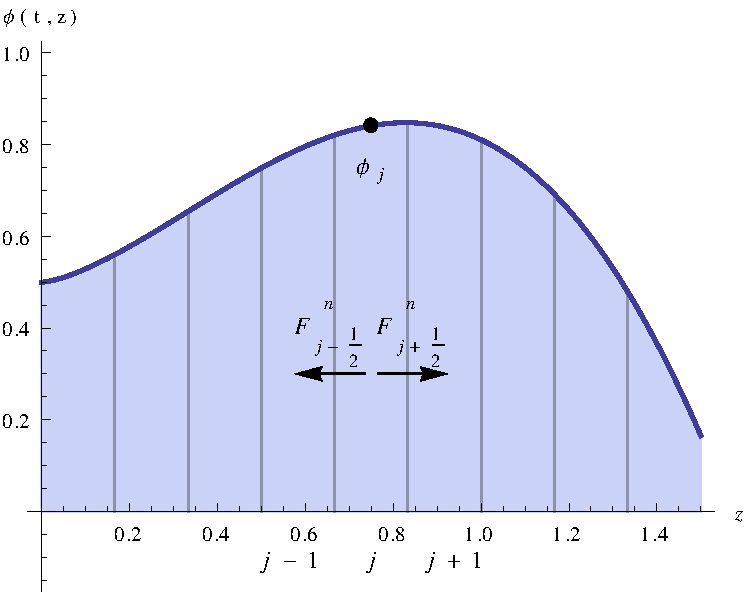
\includegraphics[scale=0.65]{/home/nicolas/git/reports/M1/vector/conservative.pdf}
\caption{$x \rightarrow u(t,x)$ and its discretisation.}
\label{}
\end{figure}

We will call  $u_j^n$ the approximate value of the $u$ function at cell number $j$ after $n$ time steps. We will call the fluxes at the right and left edges of this cell $F_{j+1/2}^n$ and $F_{j-1/2}^n$\footnote{Note that by convention the subscript $j+1/2$ ( $j-1/2$) denote the value of a quantity at the right (left) $j^{\text{th}}$ cell edge.}.

What we want to do is combine these different quantities to create a numerical scheme. The simplest scheme on can think of is obtained replacing derivatives in the conservation by finite differences:
\begin{equation}
	\frac{u^{n+1}_j - u^n_j}{\Delta T} + \frac{f(u^n_{j+1}) - f(u^n_j)}{\Delta x} = 0
\end{equation} 
This scheme involves the cell at position $j$, its right neighbour at $j+1$, but not its left neighbour at $j-1$. This asymmetry between left and right can be an advantage in particular situations, for example if we know that $u$ is advected from left to right. To get rid of this asymmetry and produce a more generally adapted scheme, we can use central differencing:
\begin{equation}
	\frac{u^{n+1}_j - u^n_j}{\Delta T} + \frac{f(u^n_{j+1}) - f(u^n_{j-1})}{2\Delta x} = 0
\end{equation}
However one can show that this scheme is unstable. The simplest generally adapted and stable scheme has been proposed for the first time by Lax and Friedrichs  in \cite{lxf}.
\section{The Lax and Friedrichs scheme}

To get the Lax and Friedrichs scheme from the above equation, we simply replace $u^n_j$ by the mean value over the left and right cells:
\begin{equation}
		\frac{u^{n+1}_j - \frac{  u^n_{j+1} + u^n_{j-1}  }{ 2 } }{\Delta T} + \frac{f(u^n_{j+1}) - f(u^n_{j-1})}{2\Delta x} = 0
\end{equation}
It can be shown that this scheme is stable\footnote{If the so-called Courant-Friedrich-Levy condition is statisfied. Essentially, the ratio of the spatial and temporal discretisation $\Delta x/ \Delta t$ must be chosen greater than the local advection speed.}. Rearranging the different terms, we can write the scheme in \textit{conservative form}:
\begin{equation}
	u^{n+1}_j = u^n_j - \frac{\Delta t}{\Delta x} \left( F^n_{j+1/2}  - F^n_{j+1/2} \right) 
\end{equation}
with
\begin{equation}
	F^n_{j+1/2} = \frac{1}{2} \left( f(u^n_{j+1}) + f(u^n_{j}) \right) - \frac{1}{2} \frac{\Delta x}{\Delta t} \left( u^n_{j+1} - u^n_{j-1} \right)
\end{equation}
The numerical fluxes $F^n_{j+1/2}$ and $F^n_{j-1/2}$ are numerical approximations of the real flux of $u$ at the edges of cell number $j$.
The Lax and Friedrichts scheme is only first-order accurate. To have a better accuracy, one can find better numerical approximations $F^n_{j \pm 1/2}$ of the flux. 

\section{The Kurganov and Tadmor scheme}

The scheme elaborated by Kurganov and Tadmor (cf \cite{KT}) can be seen as a modified version of the Lax and Friedrichs scheme approximating better the flux function. 
The idea is to evaluate numerically the value of $u$ at the edges of the cell to gain accuracy. For example the value at the right edge of cell number $j$, which we call $u^n_{j+1/2}$ accordingly to our notation, will be computed using
\begin{equation}
	u^n_{j+1/2} = u^n_j + \frac{\Delta X}{2}  \p{}{x} u^n_j
\end{equation}
where the partial derivative is computed using a finite difference formula.
Note that unless our finite differences are perfectly accurate, $u^n_{j+1/2} \neq u^n_{(j+1) - 1/2}$!
The numerical flux is now
\begin{equation}
	F^n_{j+1/2} = \frac{1}{2} \left( f(u^n_{j+1/2}) + f(u^n_{(j+1)-1/2}) \right) - \frac{1}{2} | a^n_{j+1/2} | \left( u^n_{(j+1)-1/2} - u^n_{j+1/2} \right)
\end{equation}
Note that the term $\Delta x/\Delta t$ has been replaced by the local advection speed $| a_{j+1/2}^n|$. This also plays a key role in ensuring the accuracy of the scheme.

The Kurganov and Tadmor scheme is remarkably simple, accurate and stable. 
If we chose a correct finite difference formula to compute the derivatives appearing in the edges values of $u$, the scheme can be shown to be second order accurate. That means that shocks, frequently appearing in the solutions of conservation laws, will be well resolved. It also exhibits the important \textit{total variation diminishing property}, which ensures that no oscillations will appear near the shocks. 


\chapter{Programming}
\label{app:prog}

In this appendix, I briefly present the code I developed during this internship.
The program was done in \ttt{C++}. As object-oriented programming is extensively used, rather than giving the code detailed working scheme, I will sum up its class structure. The entire code source is available here: \url{https://github.com/Yukee/flume/tree/3D/KT_solver}. 

\section {Containers}

Numerical data and equations are stored in objects called \textit{containers}.

\subsection{Scalar fields}

\begin{figure}[htp]
\centering
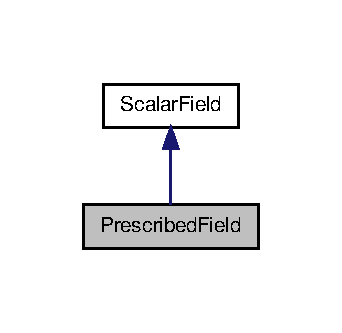
\includegraphics[scale=1.00]{appendix/class_prescribed_field__inherit__graph.pdf}
\caption{}
\label{}
\end{figure}

Numerical data is stored in objects of the \ttt{PrescribedField} class. This class derives from the \ttt{ScalarField} class. 
A \ttt{ScalarField} object represents a scalar field sampled on a discrete grid.
Two such object can be added, multiplied the same way scalar fields can. 
\ttt{ScalarField} are used for example to store the concentration, $\phi$, sampled on the integration grid.
\ttt{PrescribedField} objects are derived from \ttt{ScalarField}. In addition to behaving as scalar fields, \ttt{PrescribedField} objects can store informations about the boundary conditions at the surface bounding the domain of definition of the scalar field.
 One can \textit{prescribe} the value of the field (Dirichlet boundary condition) or the value of its derivative normal to the surface (Von Neumann boundary condition).
 
For testing purposes, I also used \ttt{PeriodicField} objects, behaving like scalar fields with periodic boundary conditions.

\subsection{Flux functions}

\begin{figure}[htp]
\centering
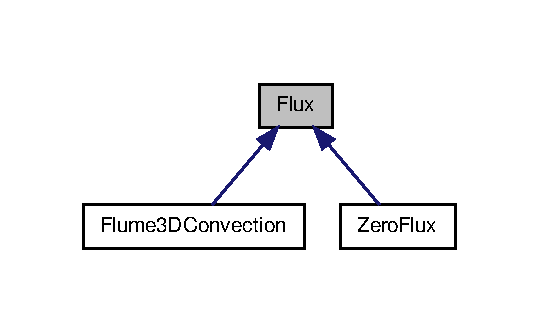
\includegraphics[scale=1.00]{appendix/class_flux__inherit__graph.pdf}
\caption{}
\label{flux}
\end{figure}

\ttt{Flux} objects behave like functions. They are used to store the information about what is the flux function $f$ (cf appendix \ref{app:finite} for the definition) in the conservation law we want to solve.
If we want to construct a new flux function, we just have to derive the base class (figure \ref{flux}).

\subsection{Equations}

\ttt{Equation} objects are used to store informations about the equation we want to solve numerically, namely
\begin{equation}
	\p{}{t} \phi + \p{}{x} f(\phi, x) = \p{}{x} D \left( \phi, \p{\phi}{x} \right) + S(\phi, x)
\end{equation}

An \ttt{Equation} stores the form of the advection flux $f$, of the diffusion flux $D$ and of the source term $S$ in \ttt{Flux} objects.

Note that this equation is slightly different from a conservation law, because of the addition of the source term $S$ and the diffusion term $D$, but it can be solved in the same way. 
A source term appear for example when we solve the 2D segregation equation in the centre plane, as explained in chapter 2. 
A diffusion flux will appear if we wish to model the effect of viscosity on the granular flow. It was not used during the internship, but can be handled by the program, and may be used in the future.

\section{Solvers}

\begin{figure}[htp]
\centering
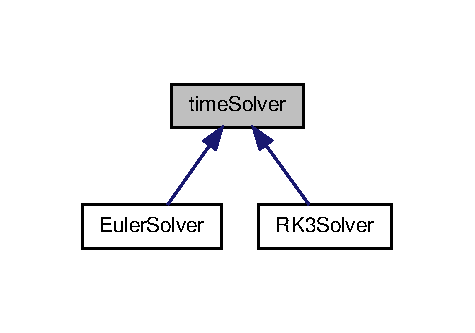
\includegraphics[scale=1.00]{appendix/classtime_solver__inherit__graph.pdf}
\caption{}
\label{}
\end{figure}

Solvers are objects designed to integrate the above equation. 
To do the time evolution, the \ttt{timeSolver} calls repetitively the \ttt{KTSolver}, whose role is to compute the numerical fluxes at the edges of the cells (cf appendix \ref{app:finite}).

For time stepping, we used the simple Euler method, and the more sophisticated order three Runge-Kutta method. 
If we want to construct a new method, we just have to derive the \ttt{timeSolver} class.

I would like to insist on the fact that the program is very general. It is able to solve any system of laws of the type (1.1), in any number of spatial dimensions.

\section{Another approach}
At the end of my internship, I created a new code based on a totally different approach. 
The base container of this new code was the \ttt{Cell}. A \ttt{Cell} object represent a finite volume cell (cf appendix ??). It contains the value of the solved field, and the values of the numerical fluxes at its edges.
A \ttt{CellArray} object stores the cells forming the integration domain. 

This approach is powerful, especially for handling boundary conditions. for example, if we want to prescribe the flux to be zero at the boundary of the domain, we just have to create a new class \ttt{BoundaryCell} derived from \ttt{Cell}, and taking into account this specificity. The \ttt{CellArray} object will then contain an heterogeneous collection of \ttt{Cell} objects (forming the inner part of the integration domain) and \ttt{BoundaryCell} objects (forming the boundary of the integration domain).

Using this approach, it is also very easy to use different numerical schemes to integrate the differential equation. I was thus able to test a number of different approaches. The source code is available here: \url{https://github.com/Yukee/finite-volume/tree/master/KT_new_1D}.

\documentclass[11pt]{article}
%Gummi|061|=)
\title{\textbf{Characteristics}}
\author{Nicolas}
\date{}
\usepackage{graphicx}
\usepackage{amsmath}
\usepackage[left=2cm,right=2cm,top=2cm,bottom=2cm]{geometry}
\newcommand{\p}[2]{\ensuremath{\frac{\partial {#1}}{\partial {#2}}}}
\newcommand{\hphi}{\ensuremath{\hat{\phi}}}

\begin{document}

\maketitle

\section{Goal and idea}
We want to solve the segregation equation
\begin{equation} \label{eq:conservative_form}
	\p{\phi}{t} + \p{u\phi}{x} + \p{v\phi}{y} + \p{w\phi}{z} - \p{\phi(1-\phi)}{z} = 0
\end{equation}

We are looking for a steady-state solution in the frame travelling at the (constant) speed of the front $u_F$. So by making the change of variable $ x \leftarrow x - u_F t$ we are left with

\begin{equation}
	\p{u\phi}{x} + \p{v\phi}{y} + \p{w\phi}{z} - \p{\phi(1-\phi)}{z} = 0
\end{equation}
We can make use of incompressibility, to take the velocity components out of the partial derivatives:
\begin{equation}
	u\p{\phi}{x} + v\p{\phi}{y} + w\p{\phi}{z} - \p{\phi(1-\phi)}{z} = 0
\end{equation}
and since $v = 0$ in the centre plane, we have
\begin{equation} \label{eq:segreg}
	u\p{\phi}{x} + w\p{\phi}{z} - \p{\phi(1-\phi)}{z} = 0
\end{equation}

Our goal is to find a solution of this equation. 
This is not an easy problem, because \cite{eq:segreg} is a \textit{partial derivatives equation}, and we have very few tools at our disposal to solve exactly this kind of differential equations.
Two things will help us. 
First, this equation can be seen as a \textit{conservation law}. Indeed if we call $\mathbf{\hat{u}}$ the velocity field 
\begin{equation}
	\mathbf{\hat{u}} = 
	\begin{pmatrix}
	u\\
	v\\
	w - (1 -\phi)\\
	\end{pmatrix}
\end{equation}
we can rewrite \cite{eq:conservative_form} as
\begin{equation}
	\p{\phi}{t} + \mathbf{\nabla} \cdot (\mathbf{\hat{u}} \phi) = 0
\end{equation}
Now we can see that the concentration in small particles,  $\phi$ is a \textit{conserved quantity} for which the flux is $\mathbf{\hat{u}} \phi$. In other words, small particles are advected without diffusion at speed $\mathbf{\hat{u}}$. 
Conservation laws can be solved using the \textit{method of the characteristics}.

\subsection{Method of the characteristics}
We can rewrite \cite{eq:segreg} as 
\begin{equation} \label{eq:carac_form}
		u\p{\phi}{x} + w\p{\phi}{z} - (1 - 2\phi)\p{\phi}{z} = 0
\end{equation}
The steady-state solution is a function of 2 variables: $ \phi = \phi(x, z)$. So the solution can be seen as the surface $ \phi - \phi(x,z) = 0$ of the 3D space $(x, z, \phi)$. 
Characteristics are curves $\phi = \hphi(x(s),z(s))$ lying on this surface, and verifying
\begin{equation}
	\frac{d \hphi}{d s} = 0
\end{equation}
Using chain rule we have 
\begin{equation}
	\p{x}{s} \p{\hphi}{x} + 
	\p{z}{s}\p{\hphi}{z} = 0
\end{equation} 
and since $\hphi$ is lying on the solution surface,
\begin{flalign}
\p{x}{s} = u \\
\p{z}{s} = w - (1- 2 \phi)
\end{flalign}
Secondly, conservation laws can easily be solved numerically with great accuracy. Solving numerically the problem gives us a useful insight (\cite{fig:1}).
\begin{figure}[htp]
\centering
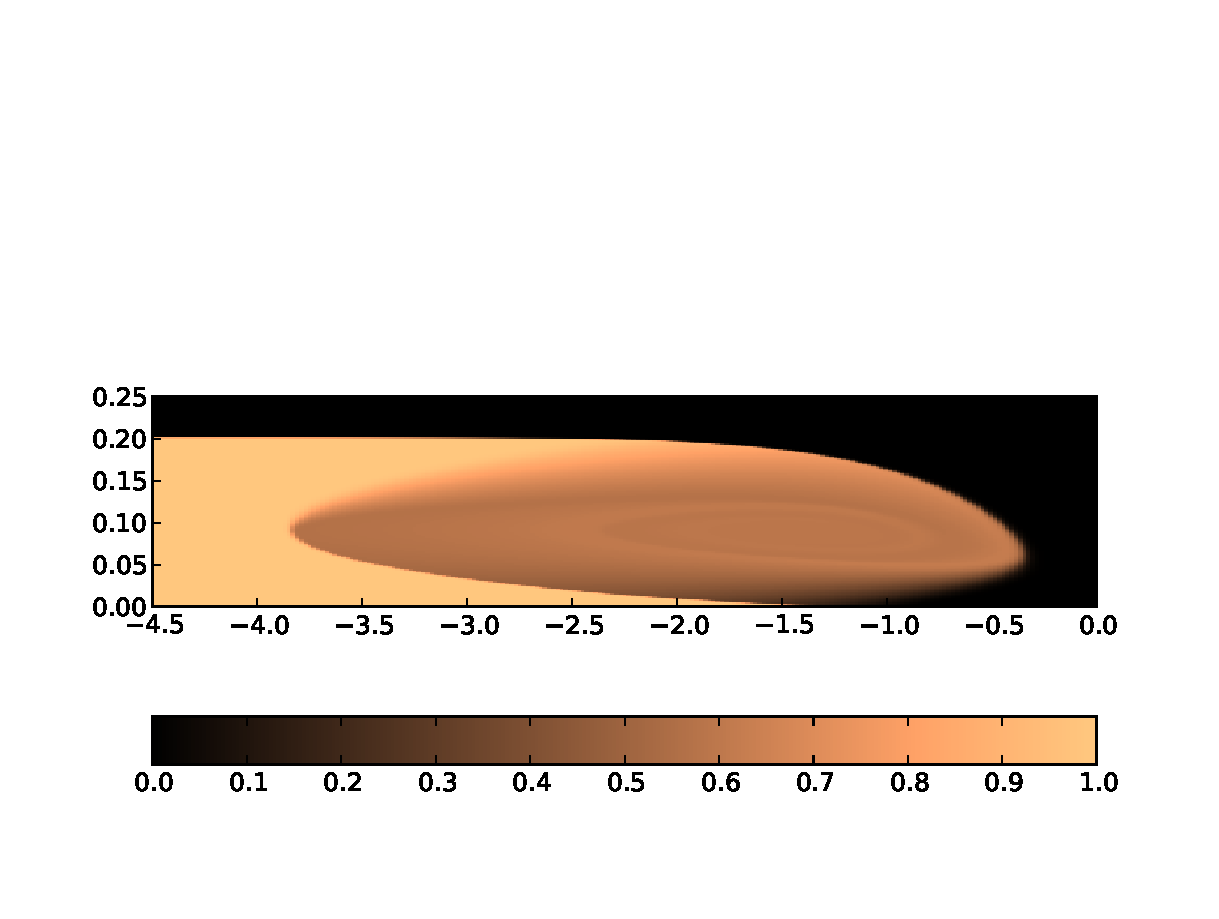
\includegraphics[scale=0.70]{spiral.pdf}
\caption{From the numerically computed steady-state solution we can deduce the general structure of the steady-state.}
\label{fig:1}
\end{figure}


\end{document}
 
% Bibliography:
\clearpage
\bibliography{bib/bib.bib}{}
\bibliographystyle{plain}
 
\end{document}